In this section we will report some results obtained by training the neural
model and applying it to an MPC based trajectory tracking problem. 

\subsection{Derivative Prediction}

In figure \ref{fig:derivative_loss} we can observe that the loss converges
pretty quickly.

\begin{figure}[H]
    \centering
    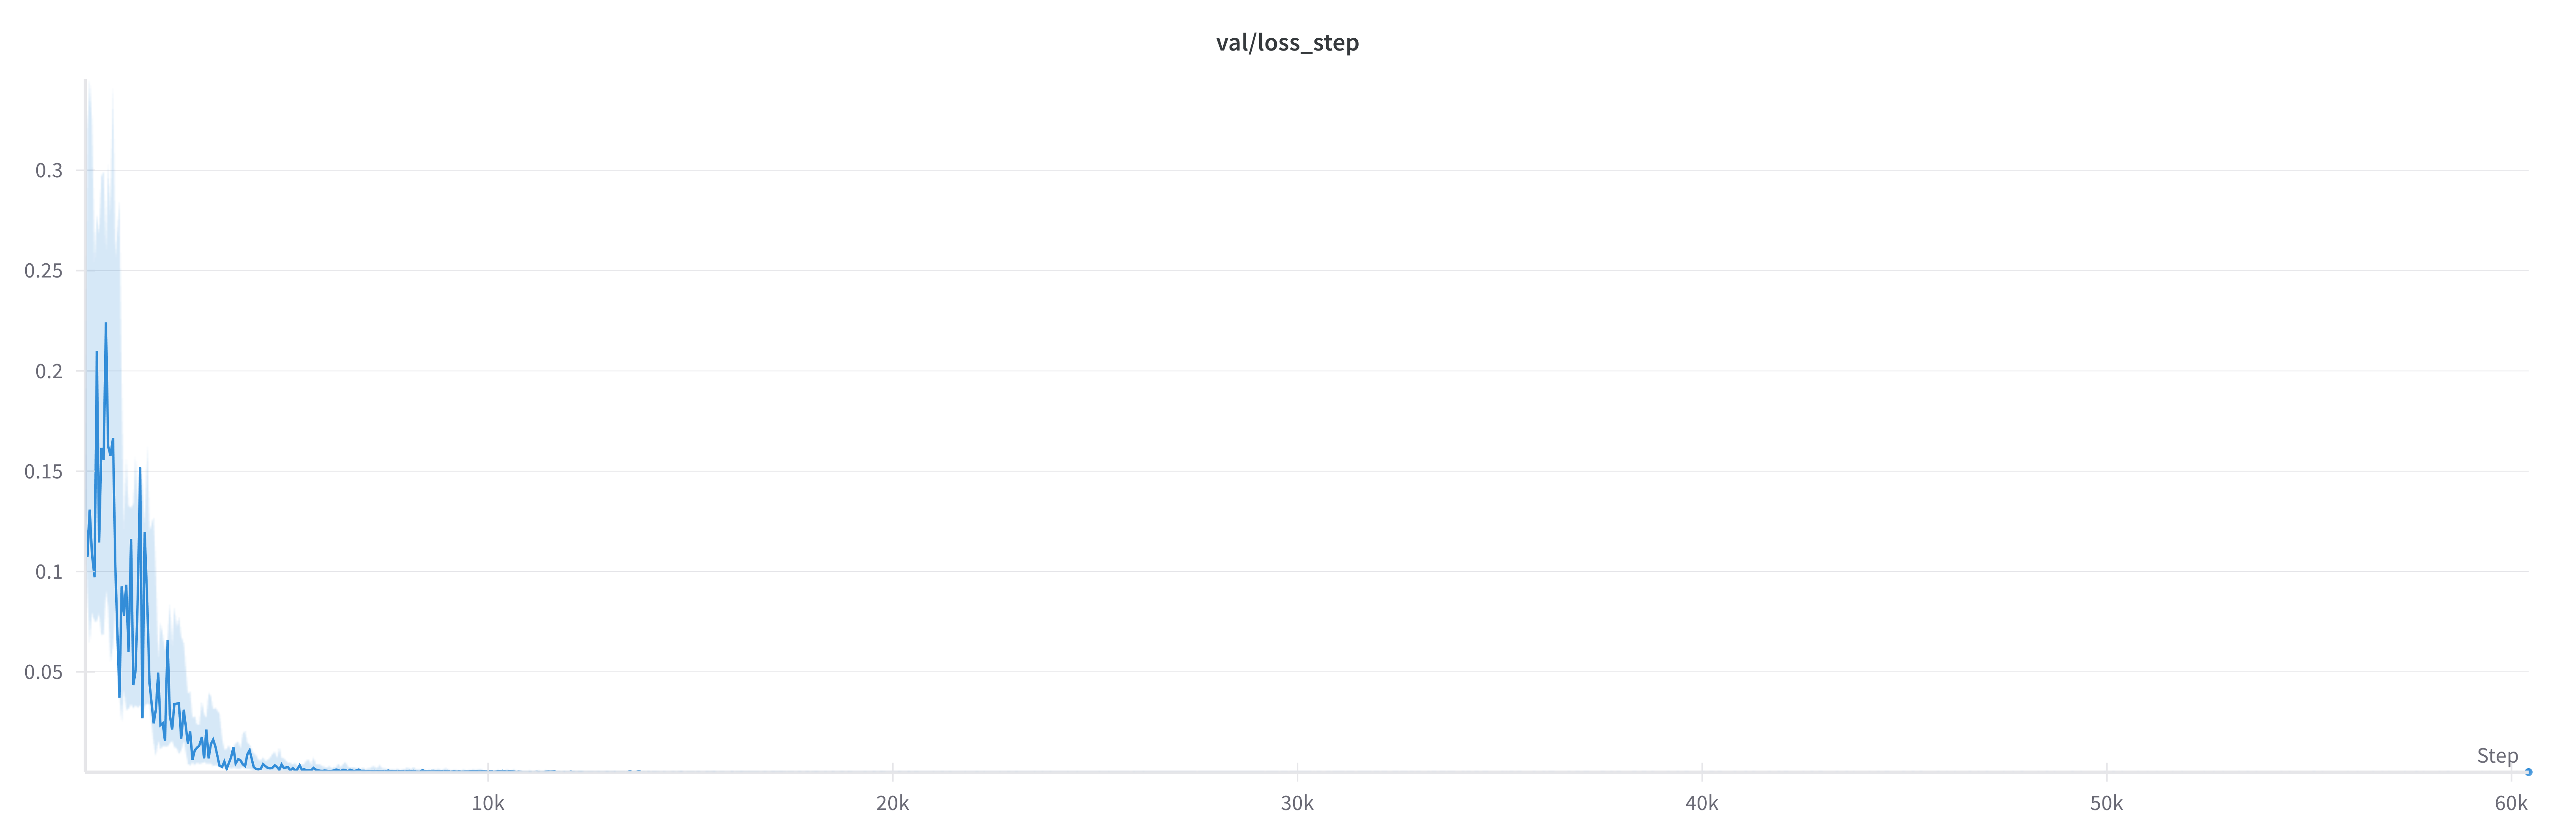
\includegraphics[width=0.8\textwidth]{assets/val_loss_derivative.png}
    \caption{Loss plot for the derivative prediction task}
    \label{fig:derivative_loss}
\end{figure}

This reflects also in a successful evaluation on the test set, where
predictions are very close to the nominal model, with very few exceptions.
Also the integration in the MPC is successful, achieving nearly identical
results to the nominal model. 

\begin{figure}[H]
    \centering
    \begin{subfigure}[b]{0.48\textwidth}
        \centering
        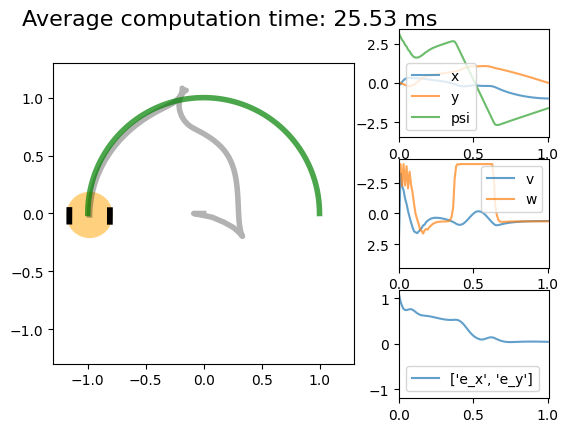
\includegraphics[width=\textwidth]{assets/mpc_neural_circle.png}
        \caption{MPC tracking with learned model}
        \label{fig:mpc_derivative_circle_1}
    \end{subfigure}
    \hfill
    \begin{subfigure}[b]{0.48\textwidth}
        \centering
        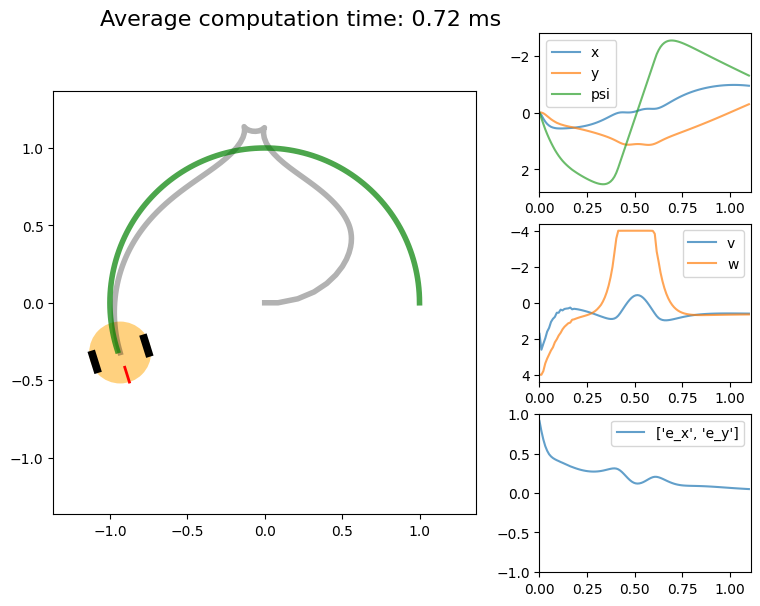
\includegraphics[width=\textwidth]{assets/mpc_nominal_circle.png}
        \caption{MPC tracking with nominal model}
        \label{fig:mpc_derivative_circle_2}
    \end{subfigure}
    \caption{Derivative prediction evaluation}
    \label{fig:mpc_derivative_circle}
\end{figure}

In these plots, the MPC simulation has a discretization timestep of 50 ms,
in order to make the neural-mpc controller feasible, since it has higher
computational demands than the nominal model. Of course, in this ideal
setting, the nominal model performs better in computational terms, but the
neural model is potentially more robust to disturbances and model errors,
especially if we were to inject noise in it during the training process.
The neural model is also potentially more scalable, since it can be trained
on a variety of more complex models, while potentially keeping the same
computational cost.


\begin{figure}[H]
    \centering
    \begin{subfigure}[b]{0.48\textwidth}
        \centering
        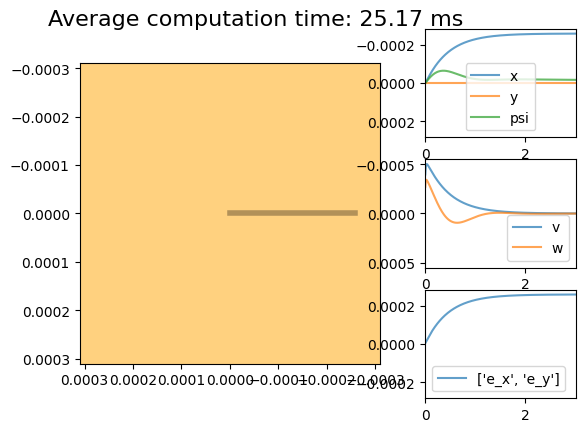
\includegraphics[width=\textwidth]{assets/mpc_neural_zero.png}
        \caption{Zero velocity testing with neural model}
    \end{subfigure}
    \hfill
    \begin{subfigure}[b]{0.48\textwidth}
        \centering
        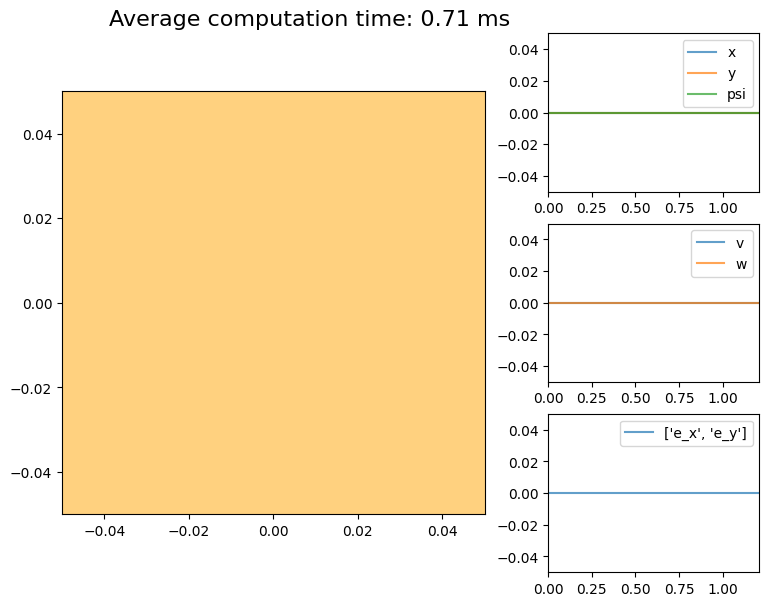
\includegraphics[width=\textwidth]{assets/mpc_nominal_zero.png}
        \caption{Zero velocity testing with nominal model}
    \end{subfigure}
    \caption{Derivative prediction evaluation}
    \label{fig:mpc_derivative_zero}
\end{figure}

In figure \ref{fig:mpc_derivative_zero} we can see that the neural model
has some issues when the desired tracking velocity is zero. The neural mpc
has a imperceptible drift, while the nominal model is, of course,
completely still. This derives from the intrisic data-related nature of
neural model, which can't captivate the differential equations profoundly.

\begin{figure}[H]
    \centering
    \begin{subfigure}[b]{0.48\textwidth}
        \centering
        \missingfigure{text}
        % 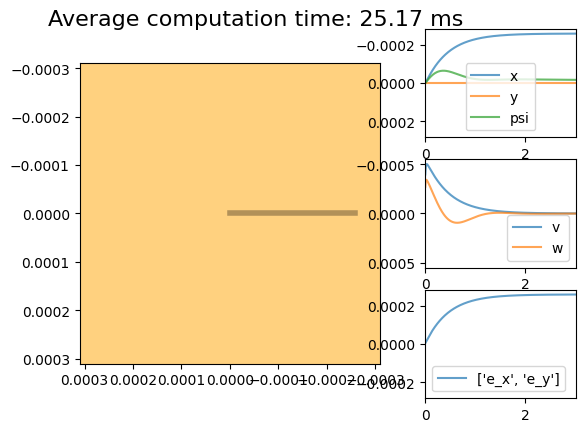
\includegraphics[width=\textwidth]{assets/mpc_neural_zero.png}
        \caption{Straight line tracking with low weight on $\omega$}
    \end{subfigure}
    \hfill
    \begin{subfigure}[b]{0.48\textwidth}
        \centering
        \missingfigure{text}
        % 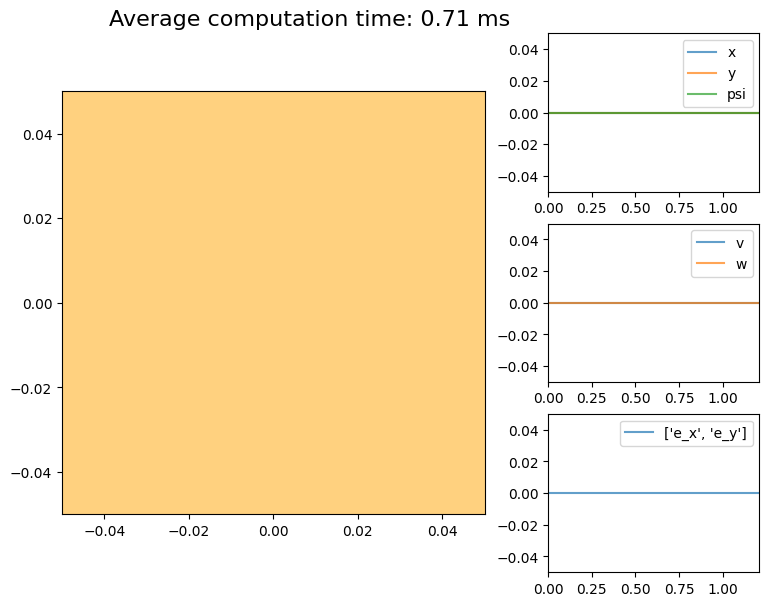
\includegraphics[width=\textwidth]{assets/mpc_nominal_zero.png}
        \caption{Straight line tracking with high weight on $\omega$}
    \end{subfigure}
    \caption{Testing two weight configurations when tracking a straight line}
    \label{fig:mpc_derivative_changing_weight}
\end{figure}


\subsection{State Prediction}

The loss for the state prediction task is depicted in figure
\ref{fig:state_loss}. The trend is very similar to before.

\begin{figure}[H]
    \centering
    \missingfigure{Loss plot for the state prediction task}
    % \includegraphics[width=0.8\textwidth]{media/state_loss.png}
    \caption{Loss plot for the state prediction task}
    \label{fig:state_loss}
\end{figure}

Similarly to before, this reflects positively in the evaluation on the
test, but there are some edge cases where dictions are not as accurate as
before. This probably comes from the fact that we use Euler integration to
propagate the nominal system dynamics. 


\begin{figure}[H]
    \centering
    \missingfigure{Unsuccesful evaluation on a test sample}
    % \includegraphics[width=0.8\textwidth]{media/state_loss.png}
    \caption{Unsuccesful evaluation on a test sample}
    \label{fig:edge_case}
\end{figure}


\begin{figure}[H]
    \centering
    \begin{subfigure}[b]{0.48\textwidth}
        \centering
        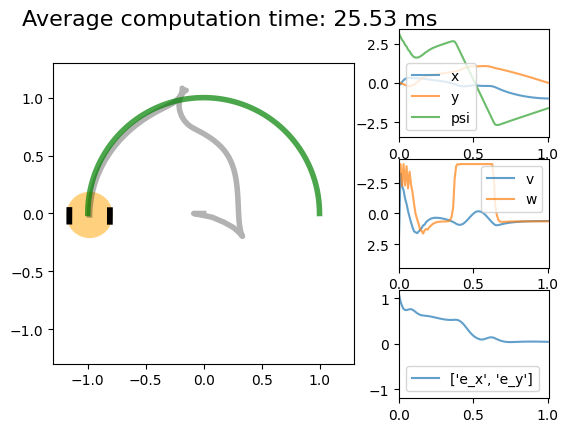
\includegraphics[width=\textwidth]{assets/mpc_neural_circle.png}
        \caption{MPC tracking with learned model}
        \label{fig:mpc_state_circle_1}
    \end{subfigure}
    \hfill
    \begin{subfigure}[b]{0.48\textwidth}
        \centering
        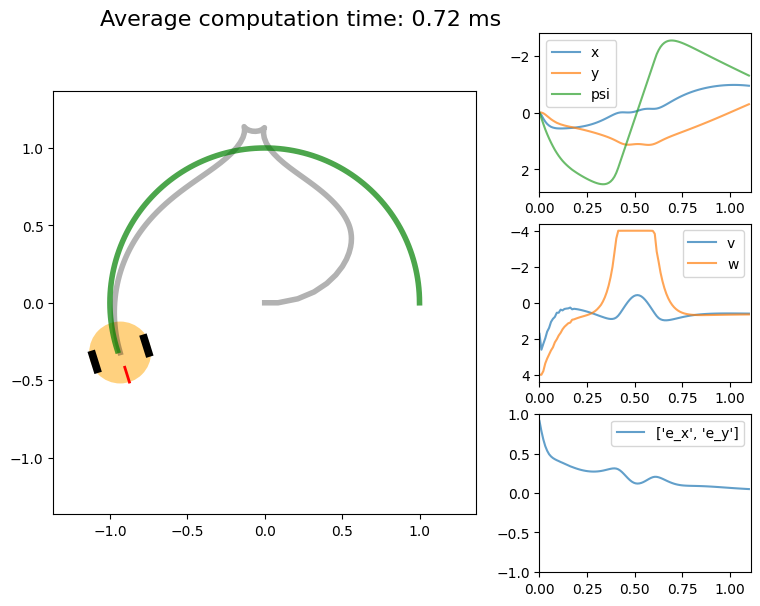
\includegraphics[width=\textwidth]{assets/mpc_nominal_circle.png}
        \caption{MPC tracking with nominal model}
        \label{fig:mpc_state_circle_2}
    \end{subfigure}
    \caption{state prediction evaluation}
    \label{fig:mpc_state_circle}
\end{figure}

The neural state prediction mpc performs better in computational terms,
probably because acados handles bettere the discrete integration rather
than ERK or Euler. On the other hand, the mpc weights need to be higher in
order 

\begin{figure}[H]
    \centering
    \begin{subfigure}[b]{0.48\textwidth}
        \centering
        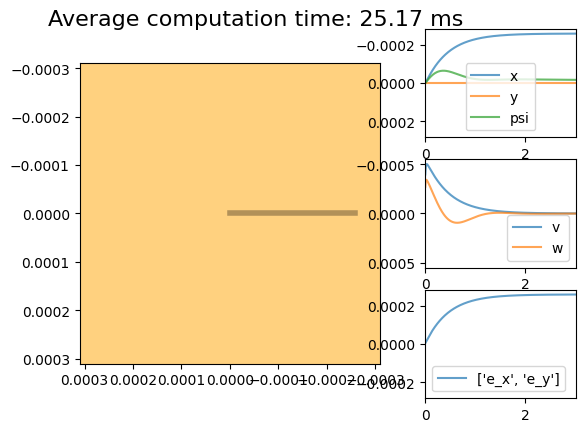
\includegraphics[width=\textwidth]{assets/mpc_neural_zero.png}
        \caption{Zero velocity testing with neural model}
    \end{subfigure}
    \hfill
    \begin{subfigure}[b]{0.48\textwidth}
        \centering
        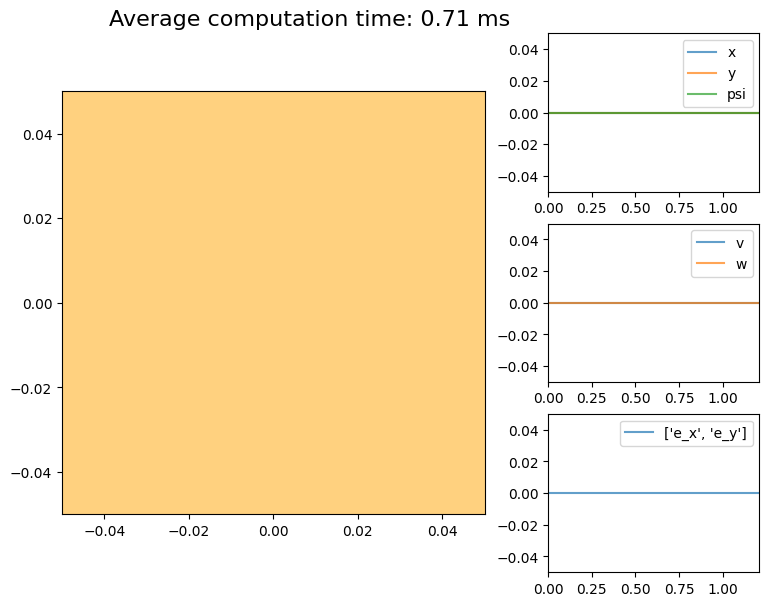
\includegraphics[width=\textwidth]{assets/mpc_nominal_zero.png}
        \caption{Zero velocity testing with nominal model}
    \end{subfigure}
    \caption{Derivative prediction evaluation}
    \label{fig:mpc_state_zero}
\end{figure}

In figure \ref{fig:mpc_state_zero} we can see that the neural model
has some issues when the desired tracking velocity is zero. The neural mpc
has a imperceptible drift, while the nominal model is, of course,
completely still. This derives from the intrisic data-related nature of
neural model, which can't captivate the differential equations profoundly.

\begin{figure}[H]
    \centering
    \begin{subfigure}[b]{0.48\textwidth}
        \centering
        \missingfigure{text}
        % 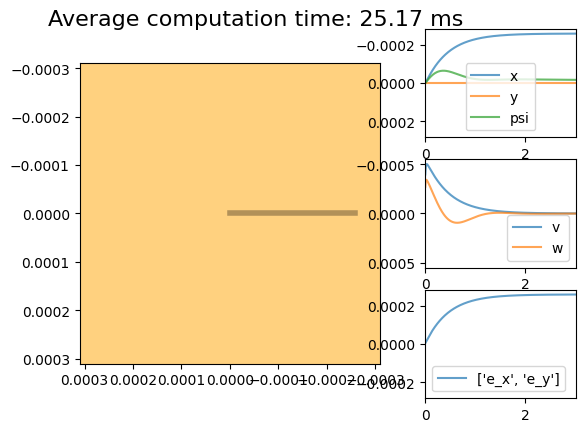
\includegraphics[width=\textwidth]{assets/mpc_neural_zero.png}
        \caption{Straight line tracking with low weight on $\omega$}
    \end{subfigure}
    \hfill
    \begin{subfigure}[b]{0.48\textwidth}
        \centering
        \missingfigure{text}
        % 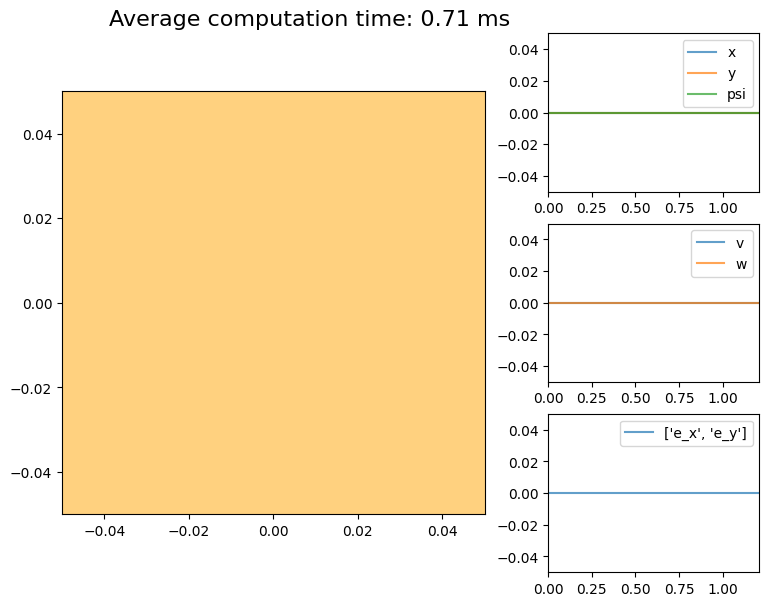
\includegraphics[width=\textwidth]{assets/mpc_nominal_zero.png}
        \caption{Straight line tracking with high weight on $\omega$}
    \end{subfigure}
    \caption{Testing two weight configurations when tracking a straight line}
    \label{fig:mpc_state_changing_weight}
\end{figure}


\subsection{State Prediction with Physics Loss}

The loss for the state prediction task is depicted in figure
\ref{fig:state_loss}. The trend is very similar to before, with a quick 

\begin{figure}[H]
    \centering
    \missingfigure{Loss plot for the state prediction task}
    % \includegraphics[width=0.8\textwidth]{media/state_loss.png}
    \caption{Loss plot for the state prediction task}
    \label{fig:pinn_loss}
\end{figure}

This reflects also in a successful evaluation on the test set, where
predictions are very close to the nominal model, with very few exceptions.
Also the integration in the MPC is successful, achieving nearly identical
results to the nominal model. 

\begin{figure}[H]
    \centering
    \begin{subfigure}[b]{0.48\textwidth}
        \centering
        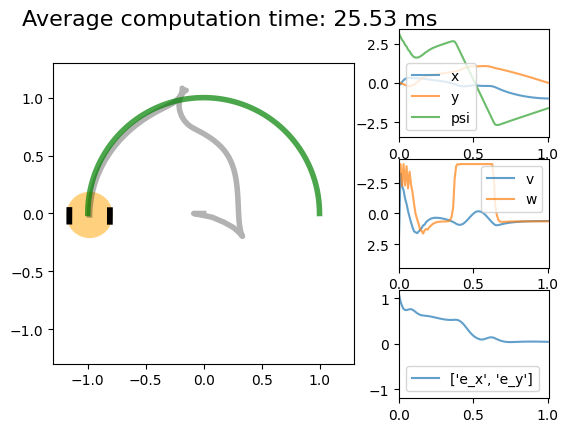
\includegraphics[width=\textwidth]{assets/mpc_neural_circle.png}
        \caption{MPC tracking with learned model}
        \label{fig:mpc_pinn_circle_1}
    \end{subfigure}
    \hfill
    \begin{subfigure}[b]{0.48\textwidth}
        \centering
        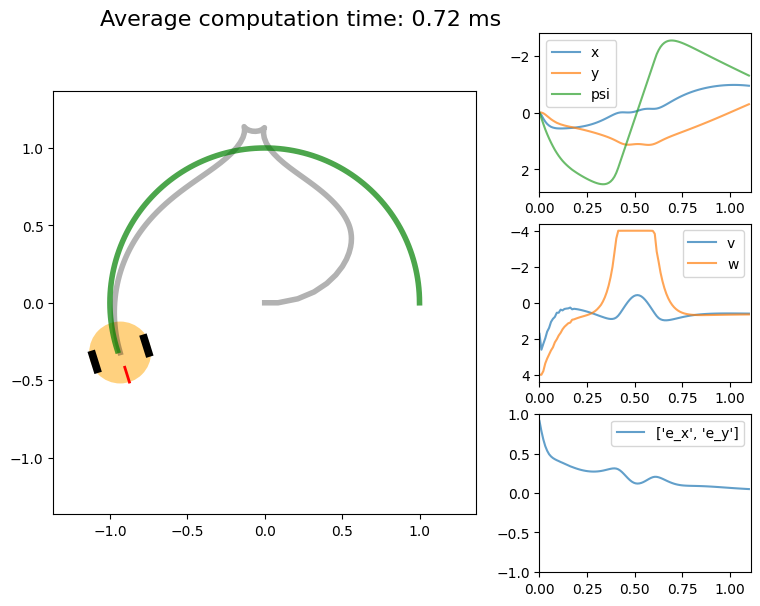
\includegraphics[width=\textwidth]{assets/mpc_nominal_circle.png}
        \caption{MPC tracking with nominal model}
        \label{fig:mpc_pinn_circle_2}
    \end{subfigure}
    \caption{pinn prediction evaluation}
    \label{fig:mpc_pinn_circle}
\end{figure}

In these plots, the MPC simulation has a discretization timestep of 50 ms,
in order to make the neural-mpc controller feasible, since it has higher
computational demands than the nominal model. Of course, in this ideal
setting, the nominal model performs better in computational terms, but the
neural model is potentially more robust to disturbances and model errors,
especially if we were to inject noise in it during the training process.
The neural model is also potentially more scalable, since it can be trained
on a variety of more complex models, while potentially keeping the same
computational cost.


\begin{figure}[H]
    \centering
    \begin{subfigure}[b]{0.48\textwidth}
        \centering
        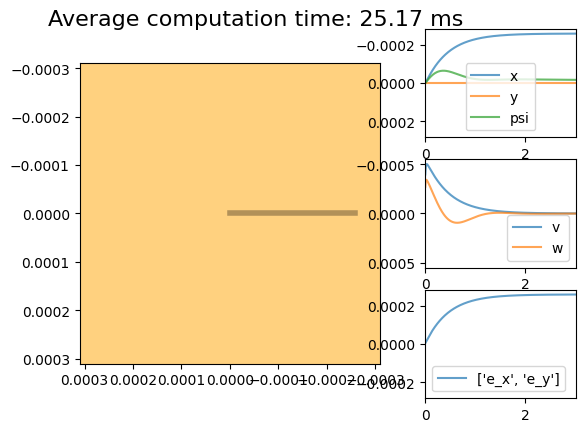
\includegraphics[width=\textwidth]{assets/mpc_neural_zero.png}
        \caption{Zero velocity testing with neural model}
    \end{subfigure}
    \hfill
    \begin{subfigure}[b]{0.48\textwidth}
        \centering
        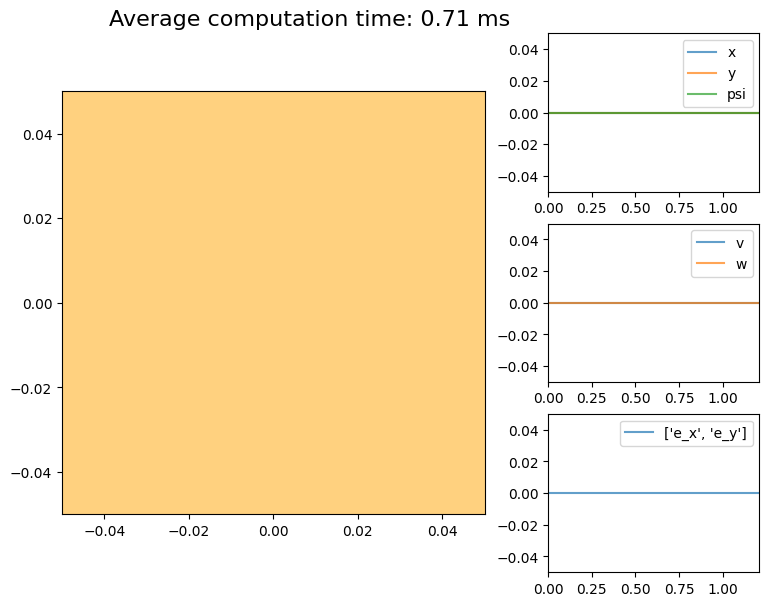
\includegraphics[width=\textwidth]{assets/mpc_nominal_zero.png}
        \caption{Zero velocity testing with nominal model}
    \end{subfigure}
    \caption{Derivative prediction evaluation}
    \label{fig:mpc_pinn_zero}
\end{figure}

In figure \ref{fig:mpc_pinn_zero} we can see that the neural model
has some issues when the desired tracking velocity is zero. The neural mpc
has a imperceptible drift, while the nominal model is, of course,
completely still. This derives from the intrisic data-related nature of
neural model, which can't captivate the differential equations profoundly.

\begin{figure}[H]
    \centering
    \begin{subfigure}[b]{0.48\textwidth}
        \centering
        \missingfigure{text}
        % 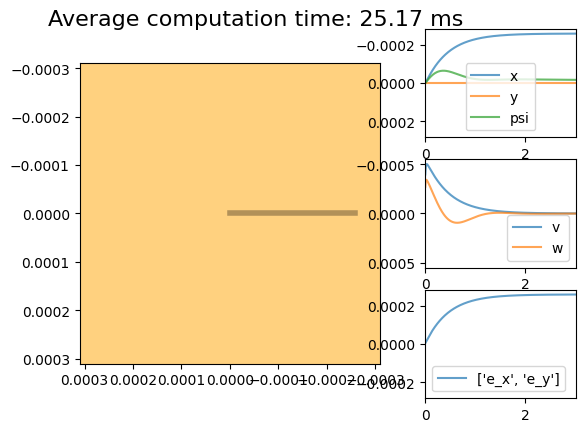
\includegraphics[width=\textwidth]{assets/mpc_neural_zero.png}
        \caption{Straight line tracking with low weight on $\omega$}
    \end{subfigure}
    \hfill
    \begin{subfigure}[b]{0.48\textwidth}
        \centering
        \missingfigure{text}
        % 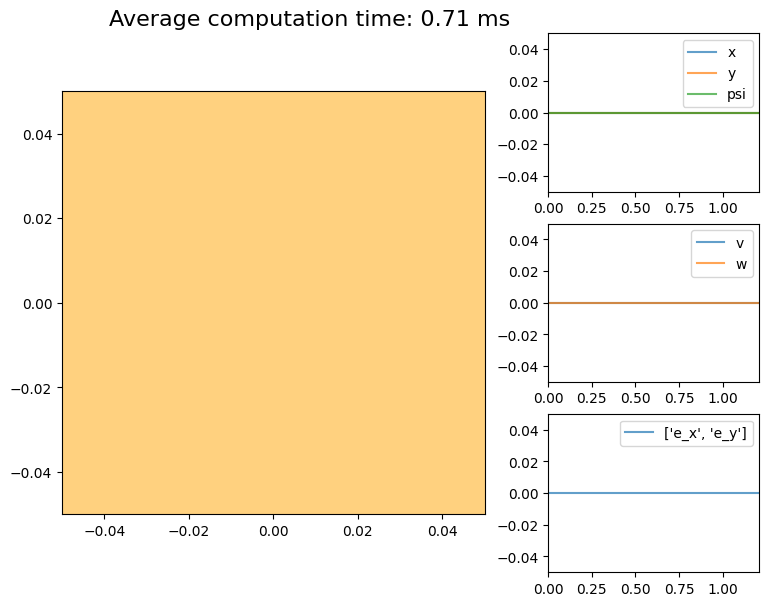
\includegraphics[width=\textwidth]{assets/mpc_nominal_zero.png}
        \caption{Straight line tracking with high weight on $\omega$}
    \end{subfigure}
    \caption{Testing two weight configurations when tracking a straight line}
    \label{fig:mpc_pinn_changing_weight}
\end{figure}